\documentclass[11pt, luatex, twoside]{book}
\usepackage{chap}



% =====================================================================
% БИБЛИОГРАФИЯ (biblatex + biber, стиль ГОСТ)
% =====================================================================
\usepackage{csquotes}% нужно для работы biblatex
\usepackage[%
backend=biber,         % движок обработки библиографии
bibencoding=utf8,      % кодировка bib-файла
sorting=none,          % порядок: по порядку цитирования (не по алфавиту)
citestyle=gost-numeric,
bibstyle=gost-numeric, % стиль по ГОСТ
clearlang=true,        % не выводить поле language, если совпадает с~языком документа
]{biblatex}
\addbibresource{lit.bib}               % файл с~библиографической базой
\setlength{\biblabelsep}{4pt}          % отступ от номера в~списке литературы
\AtBeginBibliography{\small}           % уменьшенный шрифт для списка литературы

\begin{document}

% ---------------------------------------------------------------------
% ТИТУЛ
% ---------------------------------------------------------------------
\begin{titlepage}
\thispagestyle{empty}
\vspace*{1cm}

{\headinglight\fontsize{16}{20}\selectfont Крюков П.\,А.}

\vspace{0.5cm}

{\headingfont\fontsize{32}{38}\selectfont Кинематика}

\vfill

\begin{center}
  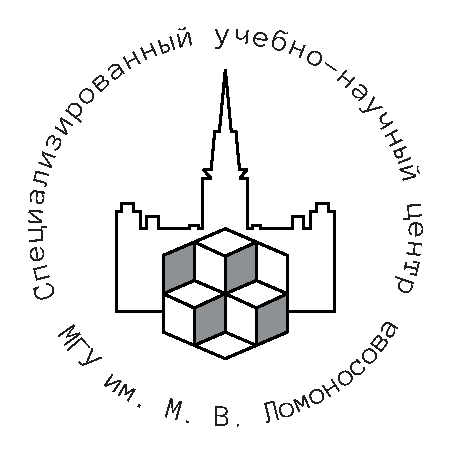
\includegraphics[width=0.6\textwidth]{images/aesc.eps}
\end{center}

\vfill

{\headinglight\fontsize{12}{16}\selectfont \the\year}

\end{titlepage}

% Оборот титула
\thispagestyle{empty}
\vspace*{\fill}
\begin{flushleft}
  \small
  Крюков П.\,А. Кинематика. \\
  \vspace{0.5\baselineskip}
  \textit{Версия от \today.}
\end{flushleft}
\clearpage

% ---------------------------------------------------------------------
% ПРЕДВАРИТЕЛЬНЫЕ СТРАНИЦЫ
% ---------------------------------------------------------------------
\frontmatter
\pagenumbering{arabic}

\tableofcontents
\clearpage

% ---------------------------------------------------------------------
% ОСНОВНОЙ ТЕКСТ
% ---------------------------------------------------------------------
\mainmatter

\chapter{Основы кинематики}
% § 4 «Задачи преследования»
\subfile{chapters/04_pursuit}

\end{document}
